\documentclass{article}

\usepackage{amsmath}
\usepackage{graphicx}

\def\I{\overline{I}}
\def\d{\mathrm{d}}
\def\x{\vec{x}}
\def\eth{\hat{e}_\theta}
\def\vnu{\vec{\nu}_{m,n}}
\def\nuth{\nu_{m,n|\theta}}
\def\pmn{\phi_{m,n}}
\def\ui{\hat{\imath}}
\def\uj{\hat{\jmath}}
\def\real{\mathrm{Re}}
\def\imag{\mathrm{Im}}

\title{A Brief Derivation for Spatial DFT Extraction from Langmuir Probe Currents}
\author{Christopher R. Martin\\Associate Professor of Mechanical Engineering\\Penn State Altoona}
\date{\today}

\begin{document}

\maketitle

\section{Introduction}

\subsection{Background}

The Langmuir probe, named for Irving Langmuir, is little more than a metal surface inserted into a plasma.  Figure \ref{fig:probe} depicts a probe with a cylindrical cross-section in a hypothetical plasma flowing from left-to-right.  When a sufficiently negative bias voltage is applied, electrons are driven away from the probe, but positive ions still impact its surface.  The result is an electrical current that may be used to deduce the density of positive ions in the fluid.  

In flames, heat transfer to the wire is sufficiently intense to destroy it, so the probes need to be actively cooled as in the famous studies by Cacote\cite{}, or the residence time in the flame must be very short as in the studies by Clements, Smy, Maclatchey, Dawe and others \cite{}.  As is evident in the latter studies, the methods used to calculate ion density in dense flowing plasmas are different from the classical methods used in sparse plasmas, but regardless of the theory used, the critical measurement is a probe surface current density at a given bias voltage.

\begin{figure}
\centering
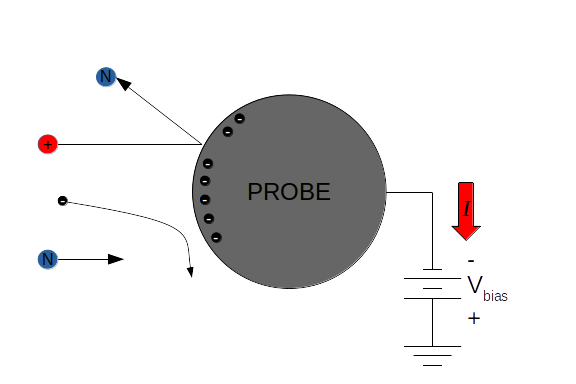
\includegraphics[width=0.97\linewidth]{figures/probe}
\caption{Example cross-section of a cylindrical Langmuir probe.  Electrons are repelled by a negative bias voltage, so currents are due to the impact of positive ions.}\label{fig:probe}
\end{figure}

For the calculations of ion density to be valid, the probe must be smaller than the length scales over which ion density changes in the fluid, but there is an essential limit to how small cylindrical probes can be before they are destroyed thermally.  For a cylinder of length, $L$, and diameter, $D$, heat transfer into the probe is proportional to $LD$.  For passive cooling, heat transfer through the probe is proportional to $D^2/L$, and for many types of active cooling, it will be proportional to $D^2$.  Regardless of the type of cooling, as $D$ diminishes, the cooling vanishes far more quickly than the rate of heating.  

Therefore, it is impractical to take high resolution Langmuir probe measurements in a dense plasma where the probe is allowed to reach its steady-state temperature.  What we will call ``transient insertion Langmuir probes'' (TILP) leave the probe in the plasma long enough to reach electrical steady-state, but briefly enough to limit the heat that enters the probe.  Spinning discs were first employed in the late twentieth century as a method to measure ion densities in dense plasmas -- specifically in flames.  However, other strategies for transient insertion are possible: a wire rapidly injected and retracted along its axis, a ceramic wheel with metal plates on its radius, a sphere on a pendulum, or even a sacrificial probe that is inserted and destroyed after the measurement is complete.

\subsection{Spatial Measurements}

In Calcote's experiments' the probe was insulated along its length except for its tip.  If the currents are guaranteed to enter at the probe's tip, the probe merely needs to be moved the locations where measurements are desired.  However, fine uninsulated wires have advantages: (1) they are much easier to fabricate, (2) they are smaller, (3) the metal resists thermal and chemical damage more easily than most insulators.  Also, if there is damage to the insulation, leakage currents can corrupt the measurement in ways that are difficult to detect.  The disadvantage is obvious; for a single measurement, there is no way to determine how the currents are distributed along the wire's length.

This work is devoted to a technique for extracting spatial information on current density from many measurements with many positions.  Provided the probe positions are carefully chosen, it is possible to reconstruct the spatial data.  While the analysis can be applied to any TILP, it is primarily derived for those mounted on spinning discs.

In the next section, we will establish the analysis, but the principle can be approached quite intuitively.  If spinning disc TILP were positioned so that the probe never enters the plasma, no current would be measured at any point of the probe's transit.  Then, if it were advanced into the plasma until the first traces of current are detected, the measured currents are certain to have come from the wire tip - the spatial location of those currents is clear.  Then, if the disc were further advanced, the probe would penetrate deeper into the plasma.  The pulse of current would broaden and grow as currents are collected at wider disc angles and over a longer length of the probe.  Rather than consider this signal on its own, we could intuitively observe that the amount by which the signal increased from the last measurement indicates the additional current encountered at the wire's tip - spatial location of the current is \emph{still} clear.  If this were repeated over the entire thickness of the plasma, a cross-section can be constructed.

\section{Derivation}

The probe wire tip protrudes a radius from the disc center, $R$, and rotates about a center at coordinates $\vec{x}_0 = x_0\ui + y_0\uj$.  At each sample, the probe has have an angle, $\theta$, enters the domain at radius, $R_0$, and terminates at a radius, $R_1$.  The current measured by the probe, $I$, is an integral of the current per unit wire length, $\I$,
\begin{align}
I = \int_{R_0}^{R_1} \I \d r.
\end{align}
These dimensions are shown in Figure \ref{fig:coords}.  It should be noted that the upper bound of the integral, $R_1$, is shown as the radius at which it leaves the domain, but it can also be the wire tip if the wire terminates in the domain.
\begin{figure}
\centering
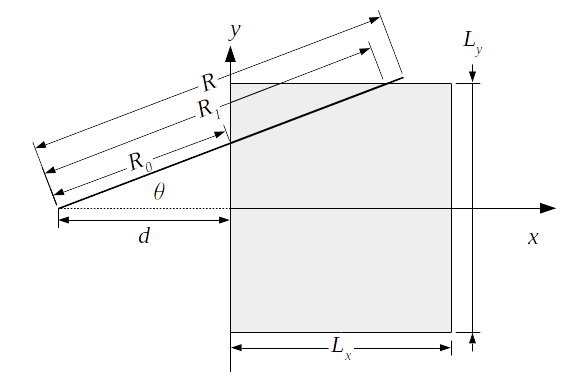
\includegraphics[width=.9\linewidth]{figures/coords}
\caption{Dimensions and coordinate system for the domain}\label{fig:coords}
\end{figure}

The wire current density is a function of the bulk velocity and the ion density, so it is expressed as a function of position in the fluid, $\I(\x)$, and may be imagined to be a local property of the fluid. 

Previously, wire current density was calculated as a grid of discrete nodes, and its integral along the wire length was calculated by interpolating along its path.  This approach is intuitive and flexible, and the inversion problem results in a sparse symmetrical matrix, which can speed inversion times.  On the other hand, the path tracing algorithm required iteration along the wire's length, which is slow in high-level languages, the discretization scheme produces artifacts in the images, and there were also unexplained striping artifacts in the wake of strong signals.

In the present work, we adopt a spatial Fourier series, which provides a far more numerically elegant formulation.

\subsection{Fourier series}

The Fourier series for $\I$ is constructed in $x,y$ coordinates
\begin{align}
\I(x,y) &= \sum_{m=-N_x}^{N_x} \sum_{n=-N_y}^{N_y} c_{m,n} \exp\left(j \vnu \cdot \x \right),\label{eqn:Ibar}
\end{align}
where $\vnu$ is the wavenumber vector,
\begin{align}
\vnu &= \nu_x \ui + \nu_y \ui\nonumber\\
 &=2\pi \left( \frac{m}{L_x} \ui + \frac{n}{L_y} \uj \right),
\end{align}
and $\x$ is the position in the domain,
\begin{align}
\x = x \ui + y \uj.
\end{align}

This formulation has $(2N_x+1)(2N_y+1)$ complex coefficients, and represents a function with periodicity $L_x$ on $x$ and $L_y$ on $y$.  It is continuous, but cannot resolve features with wavelengths shorter than $L_x / N_x$ and $L_y / N_y$.  In this way, the results are effectively spatially filtered by the highest wavenumber in the expansion.

Because the coefficients are complex-valued, each of the $(2N_x+1)(2N_y+1)$ coefficients represents two unknowns.  However, because the function, $\I$, is strictly real-valued, the coefficients must occur in complex conjugate pairs.

\subsection{Evaluating the integral}

The integral of $\I$ requires an $x,y$ parametric formulation of the wire's path.  At an angle, $\theta$, the wire is oriented along a unit vector,
\begin{align}
\hat{e}_\theta = \cos(\theta) \ui + \sin(\theta) \uj.
\end{align}

If $r$ is the distance along the wire from the disc center at $\x_0$, the corresponding location is
\begin{align}
\x &= r \eth + \x_0
\end{align}
The dot product of $\x$ and $\vnu$ yields two terms:
\begin{align}
\vnu \cdot \x &= r (\vnu \cdot \hat{e}_\theta) + (\vnu \cdot \x_0)\nonumber\\
 &= \nu_{m,n|\theta} r + \pmn\\
\nuth &= 2\pi \left( \frac{m}{L_x} \cos(\theta) + \frac{n}{L_y} \sin(\theta) \right)\\
\pmn &= 2\pi \left( \frac{m}{L_x} x_0 + \frac{n}{L_y} y_0 \right).
\end{align}
In the domain, the term still has its two-dimensional wave properties, but if we were to travel only along a wire at angle, $\theta$, the $(m,n)$ term of the expansion would appear to have wave number $\nuth$.  The second parameter, $\pmn$, is a phase that accounts for the distance along the wire to the disc center.

Later, it will be vital to note that $\nuth$ can be zero, even when both $x-$ and $y-$components of $\vnu$ are non-zero; when $\vnu$ is normal to $\eth$.  This condition is uncommon, but not impossible, so it will be vital for a well formulated code to detect it.

Once substituted into the Fourier expansion, a single term becomes
\begin{align*}
c_{m,n} \exp\left(j \vnu \cdot \x \right)\hspace{-8em}&\\
&= c_{m,n} \exp\Bigl[j \left(\nuth\,r + \pmn \right)\Bigr].
\end{align*}
Here, the disc center location, $\x_0$, appears intuitively as a phase shift.

It is convenient to define a new parameter, $\lambda_{m,n}$, which represents the value of the exponential integrated over $r$:
\begin{align}
\lambda_{m,n}(R,\x_0,\theta) &= \int_{R_0}^{R_1} \exp\Bigl[ j \left(\nuth\,r + \pmn \right)\Bigr] \d r \nonumber\\
 &= \left\{\begin{array}{c@{\ :\ }l}
 \displaystyle (R_1 - R_0) \exp\Bigl[j \pmn \Bigr] & \nuth = 0  \vspace{1.0em} \\
\displaystyle \frac{1}{j \nuth}\exp\Bigl[j \left(\nuth\,r + \pmn \right)\Bigr]^{R_1}_{R_0} & \mathrm{otherwise}
\end{array}
\right.
\end{align}
Note that we have expressed $\lambda$ as a function of the wire radius, $R$, the disc center, $\x_0$, and the wire angle relative to the $x-$axis, $\theta$.  It is worth emphasizing because all of these dependencies are implicit through $R_1$, $R_0$, $\nu_{m,n|\theta}$, and $\phi_{m,n}$.

This yields an expression for the total wire current
\begin{align}
I(R,\x_0,\theta) &= \sum_{m=-N_x}^{N_x} \sum_{n=-N_y}^{N_y} c_{m,n} \lambda_{m,n}(R,\x_0,\theta).
\end{align}

\subsection{Offset current}

Every experiment begins by zeroing the current signal to the nearest practical precision, but no real signal will ever be perfectly zero to numerical precision.  Normally, this would not be especially problematic, but the derivation above provides no representation of current sources outside of the domain.  To prevent the kinds of bizarre numerical phenomena that can occur when models awkwardly attempt to match behaviors beyond their capability, it is prudent to add a global offset parameter, $I_0$,  
\begin{align}
I(R,\x_0,\theta) &= I_0 + \sum_{m=-N_x}^{N_x} \sum_{n=-N_y}^{N_y} c_{m,n} \lambda_{m,n}(R,\x_0,\theta)\label{eqn:I}.
\end{align}


\section{Solution}

Fourier transforms classically take advantage of the orthogonality of the sinusoidal basis functions, so the original signal only needs to be integrated against each basis function over the entire domain to calculate the magnitude and phase of that component.  Because no single wire position spans the entire domain, this approach is not tenable.  Instead, a vector of coefficients must be solved by inverting a matrix.  Incidentally, the matrix inversion is not the most numerically costly part of the analysis.

The exact scheme used to organize the coefficients into a vector, $\vec{c}$, is not especially important, but it might be something along the lines of 
\begin{align}
\vec{c} = [c_{-N_x,-N_y},\ c_{-N_x+1, -N_y},\ \ldots,\ c_{-1,0},\ c_{0,0},\ c_{1,0},\ \ldots,\ c_{N_x,N_y},\ I_0]^T.
\end{align}
In this arrangement, it is equally valid to refer to a coefficient by its wavenumber indices, $c_{m,n}$, or by its place in the vector $c_k$.  When the indexing scheme above is used,
\begin{align}
k &= (m + N_x) + (n+N_y) (2N_x+1)\\
m + N_x &= k \mod{(2N_x+1)}\\
n + N_y &= \mathrm{floor}(k / (2N_x+1))
\end{align}

When the $\lambda$ values from (\ref{eqn:I}) are embedded into a second vector, $\vec{\Lambda}$, the equation may be rewritten
\begin{align}
I(R,\x_0,\theta) = \vec{\Lambda}(R,\x_0,\theta) \cdot \vec{c}.
\end{align}

For the $i$th measurement, a wire with tip at raidus, $R_i$, disc center at $\x_i$, wire at an angle $\theta_i$, and a measured wire current, $I_i$, the error between the measurement and the Fourier expansion is
\begin{align}
e_i = I_i - \vec{\Lambda}(R_i, \x_i, \theta_i) \cdot \vec{c}.
\end{align}
For compactness of notation, it will be convenient to abbreviate $\vec{\Lambda}_i = \vec{\Lambda}(R_i, \x_i, \theta_i)$ moving forward.  

Though other methods exist, least squares regression is the most common method for extracting optimal coefficients.  Using this approach, the sum of the squares of the errors, $\sum e_i{^2}$, is differentiated with respect to each of the coefficients.  When error is minimal, that differential is zero.  So,
\begin{align}
0 = \frac{\partial}{\partial c_k} \sum e_i {^2} = \sum 2\left(I_i - \vec{\Lambda}_i \cdot \vec{c}\right)\left(- \lambda_{i,k}\right).
\end{align}

Note that $\lambda_{i,k}$ is the element of $\vec{\Lambda}_i$ that corresponded to the coefficient being differentiated.  When this is repeated for each of the coefficients, and the resulting system of equations is written as a matrix problem,
\begin{align}
\vec{0} = -\sum I_i \vec{\Lambda}_i + \left(\sum \vec{\Lambda}_i \vec{\Lambda}_i{^T} \right) \vec{c}
\end{align}

The multiplication, $\vec{\Lambda} \vec{\Lambda}^T$, forms a symmetrical matrix, and the sum of many symmetrical matrices is also a symmetrical matrix.  However, because the problem is complex-valued, it is preferable to obtain a Hermitian matrix if possible.  Fortunately, it is equally valid to differentiate with respect to the complex conjugate, $\overline{c_k}$, instead of $c_k$.  This yields the problem
\begin{align}
\vec{0} = -\sum I_i \overline{\vec{\Lambda}_i}  + \left(\sum \overline{\vec{\Lambda}_i} \vec{\Lambda}_i{^T} \right) \vec{c}.
\end{align}

The sum of both the constant vector (left-hand term) and the solution matrix (right-hand term) may be accumulated over hundreds of thousands of individual measurements, so accumulating the matrix is typically a more computationally intensive task than solving the linear algebra problem.

Since there may be tens of thousands of individual wire measurements, aggregating the individual $\vec{\Lambda}$ vectors that is usually far more numerically expensive than calculating the inverse of the resulting matrix.  Fortunately, the calculation is extremely convenient to parallelize, since each measurement's contribution to the matrix and vector is independent of the others'.

\end{document}
